\documentclass[11pt,oneside]{article}

\pdfminorversion=7
\usepackage{PastProblemsStyle}

\hypersetup{
    pdftitle={Past Problems for the International Mathematical Olympiad},
    pdfauthor={Jungwoo Kim},
    pdfsubject={Past problems for the International Mathematical Olympiad},
    pdfcreator={LaTeX}
}

\begin{document}
\thispagestyle{empty}

\begin{center}
    \vspace*{1.1cm}

    {\LARGE\bfseries Past Problems\par}

    \vspace{0.25cm}

    {\large for the International Mathematical Olympiad\par}

    \vspace{0.75cm}

    {\normalsize
    Jungwoo Kim\\
    Department of Mathematics\\
    \PohangUniversityOfScienceAndTechnology
    \par}
\end{center}

\vspace{0.75cm}
\tableofcontents
\thispagestyle{empty}

\vspace{0.92cm}
\competitionpart{I}{Competition Problems}

% Official source: https://www.imo-official.org/assets/documents/problems/2015/2015_eng.pdf
\competitionyear{2015}

\begin{problem}{2015}{1}
A finite set $S$ of points in the plane is called \emph{balanced} if, for every pair of distinct points $A, B\in S$, some $C\in S$ satisfies $AC=BC$. It is called \emph{centre-free} if no point $P\in S$ satisfies $PA=PB=PC$ for three distinct points $A, B, C\in S$.
\begin{problemsubparts}
    \item Prove that a balanced set of $n$ points exists for every integer $n\ge3$.
    \item Determine all integers $n\ge3$ for which a balanced centre-free set of $n$ points exists.
\end{problemsubparts}
\end{problem}

\begin{problem}{2015}{2}
Find all triples $(a, b, c)$ of positive integers such that $ab-c$, $bc-a$, and $ca-b$ are all powers of $2$.
\end{problem}

\begin{problem}{2015}{3}
Let $ABC$ be an acute triangle with $AB>AC$, circumcircle $\Gamma$, orthocentre $H$, and altitude foot $F$ from $A$. Let $M$ be the midpoint of $BC$. Let $Q$ be the point on $\Gamma$ satisfying $\angle HQA=90^\circ$, and let $K$ be the point on $\Gamma$ satisfying $\angle HKQ=90^\circ$. Assume that $A, B, C, K, Q$ are distinct and appear on $\Gamma$ in that order.

Prove that the circumcircles of $KQH$ and $FKM$ are tangent.
\end{problem}

\begin{problem}{2015}{4}
Let $\Omega$ be the circumcircle of triangle $ABC$, with circumcentre $O$. A circle $\Gamma$ centred at $A$ meets segment $BC$ at distinct points $D, E$ in the order $B, D, E, C$. Let $F, G$ be the intersections of $\Gamma$ with $\Omega$ such that $A, F, B, C, G$ occur in this order on $\Omega$. The circumcircle of $BDF$ meets segment $AB$ again at $K$, and the circumcircle of $CGE$ meets segment $CA$ again at $L$.

Suppose that lines $FK$ and $GL$ are distinct and intersect at $X$. Prove that $X$ lies on $AO$.
\end{problem}

\begin{problem}{2015}{5}
Find all functions $f\colon\R\to\R$ for which
\[
    f(x+f(x+y))+f(xy)=x+f(x+y)+yf(x)
\]
for every $x, y\in\R$.
\end{problem}

\begin{problem}{2015}{6}
An integer sequence $(a_j)_{j\ge1}$ satisfies
\begin{problemclauses}
    \item $1\le a_j\le2015$ for every $j\ge1$;
    \item $k+a_k\ne\ell+a_\ell$ whenever $1\le k<\ell$.
\end{problemclauses}
Prove that there exist positive integers $b, N$ such that
\[
    \left|\sum_{j=m+1}^{n}(a_j-b)\right|\le1007^2
\]
for all integers $n>m\ge N$.
\end{problem}

% Official source: https://www.imo-official.org/assets/documents/problems/2016/2016_eng.pdf
\competitionyear{2016}

\begin{problem}{2016}{1}
Triangle $BCF$ is right-angled at $B$. Choose $A$ on line $CF$ so that $FA=FB$ and $F$ lies between $A$ and $C$. Point $D$ satisfies $DA=DC$, with $AC$ the bisector of $\angle DAB$. Point $E$ satisfies $EA=ED$, with $AD$ the bisector of $\angle EAC$. Let $M$ be the midpoint of $CF$, and let $X$ be chosen so that $AMXE$ is a parallelogram ($AM\parallel EX$ and $AE\parallel MX$).

Prove that $BD$, $FX$, and $ME$ are concurrent.
\end{problem}

\begin{problem}{2016}{2}
Find all positive integers $n$ for which the cells of an $n\times n$ array can be filled with the letters $I, M, O$ so that
\begin{problemclauses}
    \item in every row and column, exactly one third of the entries are each of $I$, $M$, and $O$;
    \item on every diagonal containing a multiple of $3$ cells, exactly one third of its entries are each of $I$, $M$, and $O$.
\end{problemclauses}
Here a cell is indexed by $(i, j)$, where $1\le i, j\le n$. A diagonal is the set of cells satisfying $i+j=c$ or $i-j=c$ for some constant $c$; thus both types of diagonals are included.
\end{problem}

\begin{problem}{2016}{3}
Let $P=A_1A_2\cdots A_k$ be a convex polygon whose vertices have integer coordinates and which is inscribed in a circle. Suppose that $n$ is an odd positive integer and that the squares of the side lengths of $P$ are all integers divisible by $n$. If $S$ is the area of $P$, prove that $2S$ is an integer divisible by $n$.
\end{problem}

\begin{problem}{2016}{4}
A set of positive integers is called \emph{fragrant} if it has at least two elements and each element shares a prime divisor with some other element of the set. Define $P(n)=n^2+n+1$. Determine the least positive integer $b$ for which there exists a nonnegative integer $a$ such that
\[
    \{P(a+1), P(a+2), \dots, P(a+b)\}
\]
is fragrant.
\end{problem}

\begin{problem}{2016}{5}
On a board is written the equation
\[
    (x-1)(x-2)\cdots(x-2016)
    =(x-1)(x-2)\cdots(x-2016),
\]
with $2016$ linear factors on each side. Find the smallest $k$ such that deleting exactly $k$ of these $4032$ linear factors leaves at least one factor on each side and produces an equation with no real solution.
\end{problem}

\begin{problem}{2016}{6}
There are $n\ge2$ line segments in the plane. Every two segments cross, and no three meet at one point. Geoff places a frog at one endpoint of each segment, facing the other endpoint. He then claps $n-1$ times. At every clap, each frog jumps forward to the next intersection point along its segment, without changing direction.

Geoff wants no two frogs ever to occupy the same intersection point at the same time.
\begin{problemsubparts}
    \item Prove that Geoff can always achieve this when $n$ is odd.
    \item Prove that Geoff can never achieve this when $n$ is even.
\end{problemsubparts}
\end{problem}

% Official source: https://www.imo-official.org/assets/documents/problems/2017/2017_eng.pdf
\competitionyear{2017}

\begin{problem}{2017}{1}
For an integer $a_0>1$, define the sequence $(a_n)_{n\ge0}$ by
\[
    a_{n+1}=\begin{cases}
        \sqrt{a_n}, & \text{if $\sqrt{a_n}$ is an integer}, \\
        a_n+3, & \text{otherwise}
    \end{cases}
    \qquad(n\ge0).
\]
Find all $a_0$ for which some number $A$ occurs as $a_n$ for infinitely many $n$.
\end{problem}

\begin{problem}{2017}{2}
Determine all functions $f\colon\R\to\R$ satisfying
\[
    f(f(x)f(y))+f(x+y)=f(xy)
\]
for all $x, y\in\R$.
\end{problem}

\begin{problem}{2017}{3}
A hunter and an invisible rabbit play a game in the Euclidean plane. They begin at the same point, $B_0=A_0$. After $n-1$ rounds, the rabbit and the hunter are at $A_{n-1}$ and $B_{n-1}$. The following events take place in order in round $n$:
\begin{problemchoices}
    \item The rabbit moves invisibly to $A_n$, exactly one unit from $A_{n-1}$.
    \item A tracking device announces a point $P_n$ to the hunter, with the sole guarantee that $P_nA_n\le1$.
    \item The hunter moves visibly to $B_n$, exactly one unit from $B_{n-1}$.
\end{problemchoices}
Can the hunter always choose her moves so that $A_{10^9}B_{10^9}\le100$, regardless of the rabbit's movements and the device's reports?
\end{problem}

\begin{problem}{2017}{4}
Let $R, S$ be distinct points on a circle $\Omega$ with $RS$ not a diameter, and let $\ell$ be the tangent to $\Omega$ at $R$. Point $T$ satisfies $S$ being the midpoint of $RT$. Choose $J$ on the shorter arc $RS$ of $\Omega$ such that the circumcircle $\Gamma$ of $JST$ intersects $\ell$ in two distinct points. Let $A$ be the intersection of $\Gamma$ and $\ell$ closer to $R$, and let $AJ$ meet $\Omega$ again at $K$.

Prove that $KT$ is tangent to $\Gamma$.
\end{problem}

\begin{problem}{2017}{5}
Let $N\ge2$ be an integer. A row contains $N(N+1)$ soccer players, all of different heights. Sir Alex removes $N(N-1)$ of them, leaving $2N$ players in their original order. Prove that the remaining players can be chosen so that the tallest two are adjacent, the third- and fourth-tallest are adjacent, and so on, with the shortest two also adjacent.
\end{problem}

\begin{problem}{2017}{6}
An ordered pair $(x, y)\in\Z^2$ is called a \emph{primitive point} if $\gcd(x, y)=1$. For any finite set $S$ of primitive points, prove that there exist a positive integer $n$ and integers $a_0, a_1, \dots, a_n$ such that
\[
    a_0x^n+a_1x^{n-1}y+a_2x^{n-2}y^2+\cdots+a_{n-1}xy^{n-1}+a_ny^n=1
\]
for every $(x, y)\in S$.
\end{problem}

% Official source: https://www.imo-official.org/assets/documents/problems/2018/2018_eng.pdf
\competitionyear{2018}

\begin{problem}{2018}{1}
Let $\Gamma$ be the circumcircle of an acute triangle $ABC$. Points $D\in AB$ and $E\in AC$ satisfy $AD=AE$. The perpendicular bisectors of $BD$ and $CE$ meet the minor arcs $AB$ and $AC$ of $\Gamma$ at $F$ and $G$, respectively. Prove that $DE$ and $FG$ are parallel or coincide.
\end{problem}

\begin{problem}{2018}{2}
Determine all integers $n\ge3$ for which real numbers $a_1, a_2, \dots, a_{n+2}$ exist with $a_{n+1}=a_1$, $a_{n+2}=a_2$, and
\[
    a_ia_{i+1}+1=a_{i+2}\qquad(i=1, 2, \dots, n).
\]
\end{problem}

\begin{problem}{2018}{3}
An \emph{anti-Pascal triangle} is an equilateral triangular array of numbers in which every entry outside the bottom row equals the absolute difference of the two entries directly below it. For example, the following anti-Pascal triangle of four rows contains all integers from $1$ to $10$:
\[
    \begin{array}{ccccccc}
        &&&4&&&\\
        &&2&&6&&\\
        &5&&7&&1&\\
        8&&3&&10&&9
    \end{array}
\]
Does an anti-Pascal triangle with $2018$ rows exist that contains every integer from $1$ to $1+2+\cdots+2018$?
\end{problem}

\begin{problem}{2018}{4}
A \emph{site} is a point $(x, y)$ with $x, y\in\{1, 2, \dots, 20\}$. All $400$ sites start unoccupied. Amy and Ben alternate placing stones, with Amy first. Amy places a red stone on an empty site, subject to the rule that no two red stones are at distance $\sqrt5$ from one another. Ben places a blue stone on any empty site, with no distance restriction involving blue stones. The game ends as soon as a player cannot place a stone.

Find the greatest integer $K$ for which Amy can ensure she places at least $K$ red stones, regardless of Ben's moves.
\end{problem}

\begin{problem}{2018}{5}
Let $(a_n)_{n\ge1}$ be a sequence of positive integers. Suppose there exists an integer $N\ge2$ such that
\[
    \frac{a_1}{a_2}+\frac{a_2}{a_3}+\cdots+\frac{a_{n-1}}{a_n}+\frac{a_n}{a_1}
\]
is an integer for all $n\ge N$. Prove that some positive integer $M$ satisfies $a_m=a_{m+1}$ for every $m\ge M$.
\end{problem}

\begin{problem}{2018}{6}
A convex quadrilateral $ABCD$ satisfies $AB\cdot CD=BC\cdot DA$. A point $X$ inside $ABCD$ satisfies
\[
    \angle XAB=\angle XCD, \qquad \angle XBC=\angle XDA.
\]
Prove that $\angle BXA+\angle DXC=180^\circ$.
\end{problem}

% Official source: https://www.imo-official.org/assets/documents/problems/2019/2019_eng.pdf
\competitionyear{2019}

\begin{problem}{2019}{1}
Find all functions $f\colon\Z\to\Z$ such that
\[
    f(2a)+2f(b)=f(f(a+b))
\]
for all integers $a, b$.
\end{problem}

\begin{problem}{2019}{2}
In triangle $ABC$, let $A_1\in BC$ and $B_1\in AC$. Choose $P\in AA_1$ and $Q\in BB_1$ with $PQ\parallel AB$. Point $P_1$ lies on line $PB_1$, with $B_1$ strictly between $P$ and $P_1$, and $\angle PP_1C=\angle BAC$. Similarly, point $Q_1$ lies on line $QA_1$, with $A_1$ strictly between $Q$ and $Q_1$, and $\angle CQ_1Q=\angle CBA$.

Prove that $P, Q, P_1, Q_1$ are concyclic.
\end{problem}

\begin{problem}{2019}{3}
A social network has $2019$ users with mutual friendships. The following operation may be performed repeatedly: choose users $A, B, C$ such that $A$ is friends with both $B$ and $C$, while $B$ and $C$ are not friends. Make $B$ and $C$ friends and end the friendships $AB$ and $AC$, leaving every other friendship unchanged.

Initially, $1010$ users each have $1009$ friends, and the other $1009$ users each have $1010$ friends. Prove that some sequence of the allowed operations leaves every user with at most one friend.
\end{problem}

\begin{problem}{2019}{4}
Find all pairs $(k, n)$ of positive integers satisfying
\[
    k!=(2^n-1)(2^n-2)(2^n-4)\cdots(2^n-2^{n-1}).
\]
\end{problem}

\begin{problem}{2019}{5}
The Bank of Bath issues coins marked $H$ on one side and $T$ on the other. Harry arranges $n$ such coins in a row and repeats this operation: when exactly $k>0$ coins show $H$, he flips the $k$-th coin from the left; if no coins show $H$, he stops. For instance, starting with $THT$ for $n=3$ yields
\[
    THT\to HHT\to HTT\to TTT,
\]
so the process ends after three operations.
\begin{problemsubparts}
    \item Prove that the process terminates for every initial configuration.
    \item For a configuration $C$, let $L(C)$ count the operations before termination. Thus $L(THT)=3$ and $L(TTT)=0$. Determine the average of $L(C)$ over all $2^n$ initial configurations $C$.
\end{problemsubparts}
\end{problem}

\begin{problem}{2019}{6}
Let $I$ be the incentre of an acute triangle $ABC$ with $AB\ne AC$. Its incircle $\omega$ touches $BC$, $CA$, and $AB$ at $D$, $E$, and $F$, respectively. The line through $D$ perpendicular to $EF$ meets $\omega$ again at $R$, and $AR$ meets $\omega$ again at $P$. The circumcircles of triangles $PCE$ and $PBF$ meet again at $Q$.

Prove that $DI$ and $PQ$ intersect on the line through $A$ perpendicular to $AI$.
\end{problem}

% Official source: https://www.imo-official.org/assets/documents/problems/2020/2020_eng.pdf
\competitionyear{2020}

\begin{problem}{2020}{1}
Consider the convex quadrilateral $ABCD$. The point $P$ is in the interior of $ABCD$. The following ratio equalities hold:
\[
    \angle PAD : \angle PBA : \angle DPA
    = 1:2:3 = \angle CBP : \angle BAP : \angle BPC.
\]
Prove that the following three lines meet in a point: the internal bisectors of angles $\angle ADP$ and $\angle PCB$ and the perpendicular bisector of segment $AB$.
\end{problem}

\begin{problem}{2020}{2}
The real numbers $a, b, c, d$ are such that $a\ge b\ge c\ge d>0$ and $a+b+c+d=1$. Prove that
\[
    (a+2b+3c+4d)a^ab^bc^cd^d<1.
\]
\end{problem}

\begin{problem}{2020}{3}
There are $4n$ pebbles of weights $1, 2, 3, \dots, 4n$. Each pebble is coloured in one of $n$ colours and there are four pebbles of each colour. Show that we can arrange the pebbles into two piles so that the following two conditions are both satisfied:
\begin{problemitems}
    \item The total weights of both piles are the same.
    \item Each pile contains two pebbles of each colour.
\end{problemitems}
\end{problem}

\begin{problem}{2020}{4}
There is an integer $n>1$. There are $n^2$ stations on a slope of a mountain, all at different altitudes. Each of two cable car companies, $A$ and $B$, operates $k$ cable cars; each cable car provides a transfer from one of the stations to a higher one (with no intermediate stops). The $k$ cable cars of $A$ have $k$ different starting points and $k$ different finishing points, and a cable car which starts higher also finishes higher. The same conditions hold for $B$. We say that two stations are \emph{linked} by a company if one can start from the lower station and reach the higher one by using one or more cars of that company (no other movements between stations are allowed).

Determine the smallest positive integer $k$ for which one can guarantee that there are two stations that are linked by both companies.
\end{problem}

\begin{problem}{2020}{5}
A deck of $n>1$ cards is given. A positive integer is written on each card. The deck has the property that the arithmetic mean of the numbers on each pair of cards is also the geometric mean of the numbers on some collection of one or more cards.

For which $n$ does it follow that the numbers on the cards are all equal?
\end{problem}

\begin{problem}{2020}{6}
Prove that there exists a positive constant $c$ such that the following statement is true:

Consider an integer $n>1$, and a set $S$ of $n$ points in the plane such that the distance between any two different points in $S$ is at least $1$. It follows that there is a line $\ell$ separating $S$ such that the distance from any point of $S$ to $\ell$ is at least $cn^{-1/3}$.

(A line $\ell$ \emph{separates} a set of points $S$ if some segment joining two points in $S$ crosses $\ell$.)
\end{problem}

% Official source: https://www.imo-official.org/assets/documents/problems/2021/2021_eng.pdf
\competitionyear{2021}

\begin{problem}{2021}{1}
Let $n\ge100$ be an integer. Ivan writes the numbers $n, n+1, \dots, 2n$ each on different cards. He then shuffles these $n+1$ cards, and divides them into two piles. Prove that at least one of the piles contains two cards such that the sum of their numbers is a perfect square.
\end{problem}

\begin{problem}{2021}{2}
Show that the inequality
\[
    \sum_{i=1}^{n}\sum_{j=1}^{n}\sqrt{|x_i-x_j|}
    \le \sum_{i=1}^{n}\sum_{j=1}^{n}\sqrt{|x_i+x_j|}
\]
holds for all real numbers $x_1, \dots, x_n$.
\end{problem}

\begin{problem}{2021}{3}
Let $D$ be an interior point of the acute triangle $ABC$ with $AB>AC$ so that $\angle DAB=\angle CAD$. The point $E$ on the segment $AC$ satisfies $\angle ADE=\angle BCD$, the point $F$ on the segment $AB$ satisfies $\angle FDA=\angle DBC$, and the point $X$ on the line $AC$ satisfies $CX=BX$. Let $O_1$ and $O_2$ be the circumcentres of the triangles $ADC$ and $EXD$, respectively. Prove that the lines $BC$, $EF$, and $O_1O_2$ are concurrent.
\end{problem}

\begin{problem}{2021}{4}
Let $\Gamma$ be a circle with centre $I$, and $ABCD$ a convex quadrilateral such that each of the segments $AB$, $BC$, $CD$ and $DA$ is tangent to $\Gamma$. Let $\Omega$ be the circumcircle of the triangle $AIC$. The extension of $BA$ beyond $A$ meets $\Omega$ at $X$, and the extension of $BC$ beyond $C$ meets $\Omega$ at $Z$. The extensions of $AD$ and $CD$ beyond $D$ meet $\Omega$ at $Y$ and $T$, respectively. Prove that
\[
    AD+DT+TX+XA=CD+DY+YZ+ZC.
\]
\end{problem}

\begin{problem}{2021}{5}
Two squirrels, Bushy and Jumpy, have collected 2021 walnuts for the winter. Jumpy numbers the walnuts from 1 through 2021, and digs 2021 little holes in a circular pattern in the ground around their favourite tree. The next morning Jumpy notices that Bushy had placed one walnut into each hole, but had paid no attention to the numbering. Unhappy, Jumpy decides to reorder the walnuts by performing a sequence of 2021 moves. In the $k$-th move, Jumpy swaps the positions of the two walnuts adjacent to walnut $k$.

Prove that there exists a value of $k$ such that, on the $k$-th move, Jumpy swaps some walnuts $a$ and $b$ such that $a<k<b$.
\end{problem}

\begin{problem}{2021}{6}
Let $m\ge2$ be an integer, $A$ be a finite set of (not necessarily positive) integers, and $B_1, B_2, B_3, \dots, B_m$ be subsets of $A$. Assume that for each $k=1, 2, \dots, m$ the sum of the elements of $B_k$ is $m^k$. Prove that $A$ contains at least $m/2$ elements.
\end{problem}

% Official source: https://www.imo-official.org/assets/documents/problems/2022/2022_eng.pdf
\competitionyear{2022}

\begin{problem}{2022}{1}
The Bank of Oslo issues two types of coin: aluminium (denoted $A$) and bronze (denoted $B$). Marianne has $n$ aluminium coins and $n$ bronze coins, arranged in a row in some arbitrary initial order. A \emph{chain} is any subsequence of consecutive coins of the same type. Given a fixed positive integer $k\le2n$, Marianne repeatedly performs the following operation: she identifies the longest chain containing the $k$-th coin from the left, and moves all coins in that chain to the left end of the row. For example, if $n=4$ and $k=4$, the process starting from the ordering $AABBBABA$ would be
\[
\begin{gathered}
    AAB\underline{B}BABA\to BBB\underline{A}AABA\to AAA\underline{B}BBBA\\
    \to BBB\underline{B}AAAA\to BBB\underline{B}AAAA\to\cdots.
\end{gathered}
\]
Find all pairs $(n, k)$ with $1\le k\le2n$ such that for every initial ordering, at some moment during the process, the leftmost $n$ coins will all be of the same type.
\end{problem}

\begin{problem}{2022}{2}
Find all functions $f\colon\R_{>0}\to\R_{>0}$ such that for each $x\in\R_{>0}$, there is exactly one $y\in\R_{>0}$ satisfying
\[
    xf(y)+yf(x)\le2.
\]
\end{problem}

\begin{problem}{2022}{3}
Let $k$ be a positive integer and let $S$ be a finite set of odd prime numbers. Prove that there is at most one way (up to rotation and reflection) to place the elements of $S$ around a circle such that the product of any two neighbours is of the form $x^2+x+k$ for some positive integer $x$.
\end{problem}

\begin{problem}{2022}{4}
Let $ABCDE$ be a convex pentagon such that $BC=DE$. Assume that there is a point $T$ inside $ABCDE$ with $TB=TD$, $TC=TE$ and $\angle ABT=\angle TEA$. Let line $AB$ intersect lines $CD$ and $CT$ at points $P$ and $Q$, respectively. Assume that the points $P, B, A, Q$ occur on their line in that order. Let line $AE$ intersect lines $CD$ and $DT$ at points $R$ and $S$, respectively. Assume that the points $R, E, A, S$ occur on their line in that order. Prove that the points $P, S, Q, R$ lie on a circle.
\end{problem}

\begin{problem}{2022}{5}
Find all triples $(a, b, p)$ of positive integers with $p$ prime and
\[
    a^p=b!+p.
\]
\end{problem}

\begin{problem}{2022}{6}
Let $n$ be a positive integer. A \emph{Nordic square} is an $n\times n$ board containing all the integers from $1$ to $n^2$ so that each cell contains exactly one number. Two different cells are considered adjacent if they share a common side. Every cell that is adjacent only to cells containing larger numbers is called a \emph{valley}. An \emph{uphill path} is a sequence of one or more cells such that:
\begin{problemclauses}
    \item the first cell in the sequence is a valley,
    \item each subsequent cell in the sequence is adjacent to the previous cell, and
    \item the numbers written in the cells in the sequence are in increasing order.
\end{problemclauses}
Find, as a function of $n$, the smallest possible total number of uphill paths in a Nordic square.
\end{problem}

% Official source: https://www.imo-official.org/assets/documents/problems/2023/2023_eng.pdf
\competitionyear{2023}

\begin{problem}{2023}{1}
Determine all composite integers $n>1$ that satisfy the following property: if $d_1, d_2, \dots, d_k$ are all the positive divisors of $n$ with $1=d_1<d_2<\cdots<d_k=n$, then $d_i$ divides $d_{i+1}+d_{i+2}$ for every $1\le i\le k-2$.
\end{problem}

\begin{problem}{2023}{2}
Let $ABC$ be an acute-angled triangle with $AB<AC$. Let $\Omega$ be the circumcircle of $ABC$. Let $S$ be the midpoint of the arc $CB$ of $\Omega$ containing $A$. The perpendicular from $A$ to $BC$ meets $BS$ at $D$ and meets $\Omega$ again at $E\ne A$. The line through $D$ parallel to $BC$ meets line $BE$ at $L$. Denote the circumcircle of triangle $BDL$ by $\omega$. Let $\omega$ meet $\Omega$ again at $P\ne B$.

Prove that the line tangent to $\omega$ at $P$ meets line $BS$ on the internal angle bisector of $\angle BAC$.
\end{problem}

\begin{problem}{2023}{3}
For each integer $k\ge2$, determine all infinite sequences of positive integers $a_1, a_2, \dots$ for which there exists a polynomial $P$ of the form $P(x)=x^k+c_{k-1}x^{k-1}+\cdots+c_1x+c_0$, where $c_0, c_1, \dots, c_{k-1}$ are non-negative integers, such that
\[
    P(a_n)=a_{n+1}a_{n+2}\cdots a_{n+k}
\]
for every integer $n\ge1$.
\end{problem}

\begin{problem}{2023}{4}
Let $x_1, x_2, \dots, x_{2023}$ be pairwise different positive real numbers such that
\[
    a_n=\sqrt{(x_1+x_2+\cdots+x_n)
    \left(\frac1{x_1}+\frac1{x_2}+\cdots+\frac1{x_n}\right)}
\]
is an integer for every $n=1, 2, \dots, 2023$. Prove that $a_{2023}\ge3034$.
\end{problem}

\begin{problem}{2023}{5}
Let $n$ be a positive integer. A \emph{Japanese triangle} consists of $1+2+\cdots+n$ circles arranged in an equilateral triangular shape such that for each $i=1, 2, \dots, n$, the $i$-th row contains exactly $i$ circles, exactly one of which is coloured red. A \emph{ninja path} in a Japanese triangle is a sequence of $n$ circles obtained by starting in the top row, then repeatedly going from a circle to one of the two circles immediately below it and finishing in the bottom row. Here is an example of a Japanese triangle with $n=6$, along with a ninja path in that triangle containing two red circles.

% Faithful textbook-style TikZ reconstruction of the official 2023 IMO Problem 5 example.
\begin{center}
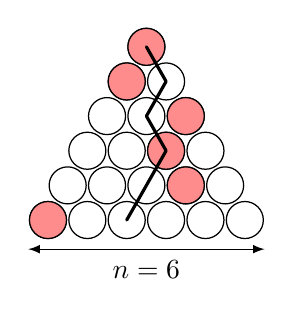
\begin{tikzpicture}[x=1cm,y=1cm,line cap=round,line join=round]
    \def\circleRadius{0.235}
    \foreach \row in {1,...,6}{
        \foreach \column in {1,...,\row}{
            \coordinate (r\row c\column) at ({(\column-(\row+1)/2)*0.50},{(6-\row)*0.44});
        }
    }
    \foreach \row in {1,...,6}{
        \foreach \column in {1,...,\row}{
            \draw[line width=0.45pt,fill=white] (r\row c\column) circle (\circleRadius);
        }
    }
    % Exactly one red circle in each row, as in the official example.
    \foreach \r/\c in {1/1,2/1,3/3,4/3,5/4,6/1}{
        \draw[line width=0.45pt,fill=red!45] (r\r c\c) circle (\circleRadius);
    }
    % A ninja path through two red circles (rows 1 and 4).
    \draw[line width=1.15pt] (r1c1.center)--(r2c2.center)--(r3c2.center)
        --(r4c3.center)--(r5c3.center)--(r6c3.center);
    \draw[latex-latex,line width=0.45pt] (-1.50,-0.37)--(1.50,-0.37);
    \node[below] at (0,-0.39) {$n=6$};
\end{tikzpicture}
\end{center}


In terms of $n$, find the greatest $k$ such that in each Japanese triangle there is a ninja path containing at least $k$ red circles.
\end{problem}

\begin{problem}{2023}{6}
Let $ABC$ be an equilateral triangle. Let $A_1, B_1, C_1$ be interior points of $ABC$ such that $BA_1=A_1C$, $CB_1=B_1A$, $AC_1=C_1B$, and
\[
    \angle BA_1C+\angle CB_1A+\angle AC_1B=480^\circ.
\]
Let $BC_1$ and $CB_1$ meet at $A_2$, let $CA_1$ and $AC_1$ meet at $B_2$, and let $AB_1$ and $BA_1$ meet at $C_2$. Prove that if triangle $A_1B_1C_1$ is scalene, then the three circumcircles of triangles $AA_1A_2$, $BB_1B_2$ and $CC_1C_2$ all pass through two common points.
\end{problem}

% Official source: https://www.imo-official.org/assets/documents/problems/2024/2024_eng.pdf
\competitionyear{2024}

\begin{problem}{2024}{1}
Determine all real numbers $\alpha$ such that, for every positive integer $n$, the integer
\[
    \lfloor\alpha\rfloor+\lfloor2\alpha\rfloor+\cdots+\lfloor n\alpha\rfloor
\]
is a multiple of $n$.
\end{problem}

\begin{problem}{2024}{2}
Determine all pairs $(a, b)$ of positive integers for which there exist positive integers $g$ and $N$ such that
\[
    \gcd(a^n+b, b^n+a)=g
\]
holds for all integers $n\ge N$.
\end{problem}

\begin{problem}{2024}{3}
Let $a_1, a_2, a_3, \dots$ be an infinite sequence of positive integers, and let $N$ be a positive integer. Suppose that, for each $n>N$, $a_n$ is equal to the number of times $a_{n-1}$ appears in the list $a_1, a_2, \dots, a_{n-1}$.

Prove that at least one of the sequences $a_1, a_3, a_5, \dots$ and $a_2, a_4, a_6, \dots$ is eventually periodic.

(An infinite sequence $b_1, b_2, b_3, \dots$ is \emph{eventually periodic} if there exist positive integers $p$ and $M$ such that $b_{m+p}=b_m$ for all $m\ge M$.)
\end{problem}

\begin{problem}{2024}{4}
Let $ABC$ be a triangle with $AB<AC<BC$. Let the incentre and incircle of triangle $ABC$ be $I$ and $\omega$, respectively. Let $X$ be the point on line $BC$ different from $C$ such that the line through $X$ parallel to $AC$ is tangent to $\omega$. Similarly, let $Y$ be the point on line $BC$ different from $B$ such that the line through $Y$ parallel to $AB$ is tangent to $\omega$. Let $AI$ intersect the circumcircle of triangle $ABC$ again at $P\ne A$. Let $K$ and $L$ be the midpoints of $AC$ and $AB$, respectively.

Prove that $\angle KIL+\angle YPX=180^\circ$.
\end{problem}

\begin{problem}{2024}{5}
Turbo the snail plays a game on a board with 2024 rows and 2023 columns. There are hidden monsters in 2022 of the cells. Initially, Turbo does not know where any of the monsters are, but he knows that there is exactly one monster in each row except the first row and the last row, and that each column contains at most one monster.

Turbo makes a series of attempts to go from the first row to the last row. On each attempt, he chooses to start on any cell in the first row, then repeatedly moves to an adjacent cell sharing a common side. (He is allowed to return to a previously visited cell.) If he reaches a cell with a monster, his attempt ends and he is transported back to the first row to start a new attempt. The monsters do not move, and Turbo remembers whether or not each cell he has visited contains a monster. If he reaches any cell in the last row, his attempt ends and the game is over.

Determine the minimum value of $n$ for which Turbo has a strategy that guarantees reaching the last row on the $n$-th attempt or earlier, regardless of the locations of the monsters.
\end{problem}

\begin{problem}{2024}{6}
A function $f\colon\Q\to\Q$ is called \emph{aquaesulian} if the following property holds: for every $x, y\in\Q$,
\[
    f(x+f(y))=f(x)+y
    \qquad\text{or}\qquad
    f(f(x)+y)=x+f(y).
\]
Show that there exists an integer $c$ such that for any aquaesulian function $f$ there are at most $c$ different rational numbers of the form $f(r)+f(-r)$ for some rational number $r$, and find the smallest possible value of $c$.
\end{problem}

% Official source: https://www.imo-official.org/assets/documents/problems/2025/2025_eng.pdf
\competitionyear{2025}

\begin{problem}{2025}{1}
A line in the plane is called \emph{sunny} if it is not parallel to any of the $x$-axis, the $y$-axis, and the line $x+y=0$.

Let $n\ge3$ be a given integer. Determine all nonnegative integers $k$ such that there exist $n$ distinct lines in the plane satisfying both of the following:
\begin{problemitems}
    \item for all positive integers $a$ and $b$ with $a+b\le n+1$, the point $(a, b)$ is on at least one of the lines; and
    \item exactly $k$ of the $n$ lines are sunny.
\end{problemitems}
\end{problem}

\begin{problem}{2025}{2}
Let $\Omega$ and $\Gamma$ be circles with centres $M$ and $N$, respectively, such that the radius of $\Omega$ is less than the radius of $\Gamma$. Suppose circles $\Omega$ and $\Gamma$ intersect at two distinct points $A$ and $B$. Line $MN$ intersects $\Omega$ at $C$ and $\Gamma$ at $D$, such that points $C, M, N$ and $D$ lie on the line in that order. Let $P$ be the circumcentre of triangle $ACD$. Line $AP$ intersects $\Omega$ again at $E\ne A$. Line $AP$ intersects $\Gamma$ again at $F\ne A$. Let $H$ be the orthocentre of triangle $PMN$.

Prove that the line through $H$ parallel to $AP$ is tangent to the circumcircle of triangle $BEF$.
\end{problem}

\begin{problem}{2025}{3}
A function $f\colon\N\to\N$ is said to be \emph{bonza} if
\[
    f(a)\mid b^a-f(b)^{f(a)}
\]
for all positive integers $a$ and $b$.

Determine the smallest real constant $c$ such that $f(n)\le cn$ for all bonza functions $f$ and all positive integers $n$.
\end{problem}

\begin{problem}{2025}{4}
A \emph{proper divisor} of a positive integer $N$ is a positive divisor of $N$ other than $N$ itself.

The infinite sequence $a_1, a_2, \dots$ consists of positive integers, each of which has at least three proper divisors. For each $n\ge1$, the integer $a_{n+1}$ is the sum of the three largest proper divisors of $a_n$.

Determine all possible values of $a_1$.
\end{problem}

\begin{problem}{2025}{5}
Alice and Bazza are playing the \emph{inekoalaty game}, a two-player game whose rules depend on a positive real number $\lambda$ which is known to both players. On the $n$-th turn of the game (starting with $n=1$) the following happens:
\begin{problemitems}
    \item If $n$ is odd, Alice chooses a nonnegative real number $x_n$ such that
    \[
        x_1+x_2+\cdots+x_n\le\lambda n.
    \]
    \item If $n$ is even, Bazza chooses a nonnegative real number $x_n$ such that
    \[
        x_1^2+x_2^2+\cdots+x_n^2\le n.
    \]
\end{problemitems}
If a player cannot choose a suitable number $x_n$, the game ends and the other player wins. If the game goes on forever, neither player wins. All chosen numbers are known to both players.

Determine all values of $\lambda$ for which Alice has a winning strategy and all those for which Bazza has a winning strategy.
\end{problem}

\begin{problem}{2025}{6}
Consider a $2025\times2025$ grid of unit squares. Matilda wishes to place on the grid some rectangular tiles, possibly of different sizes, such that each side of every tile lies on a grid line and every unit square is covered by at most one tile.

Determine the minimum number of tiles Matilda needs to place so that each row and each column of the grid has exactly one unit square that is not covered by any tile.
\end{problem}

% Official source: https://www.imo-official.org/assets/documents/problems/2026/2026_eng.pdf
\competitionyear{2026}

\begin{problem}{2026}{1}
There are 2026 integers greater than $1$ written on a blackboard, not necessarily different. In a move, Confucius chooses two integers $m>1$ and $n>1$ from different places on the blackboard and replaces these two integers with
\[
    \gcd(m, n) \qquad\text{and}\qquad
    \frac{\lcmop(m, n)}{\gcd(m, n)}.
\]
He continues to make moves while it is possible to do so.
\begin{problemsubparts}
    \item Prove that, regardless of the choices of Confucius, after finitely many moves, exactly one integer $M$ on the blackboard is greater than $1$.
    \item Prove that the value of $M$ does not depend on the choices of Confucius.
\end{problemsubparts}
\end{problem}

\begin{problem}{2026}{2}
Let $ABC$ be a triangle and let points $M$ and $N$ be the midpoints of sides $AB$ and $AC$, respectively. Let points $K$ and $L$ be chosen strictly inside triangles $BMC$ and $BNC$, respectively, such that $K$ lies strictly inside triangle $ABL$ and $L$ lies strictly inside triangle $AKC$. Suppose that
\[
    \angle KBA=\angle ACL, \qquad
    \angle LBK=\angle LNC, \qquad
    \angle LCK=\angle BMK.
\]
Let $O$ be the circumcentre of triangle $AKL$. Prove that $OM=ON$.
\end{problem}

\begin{problem}{2026}{3}
Let $n$ be a positive integer. Liu Bang and Xiang Yu have a stick of length $1$ and want to divide it between themselves. Liu marks at most $n$ points on the stick, and then Xiang marks at most $n$ points on the stick. The marked points are distinct. Then, the stick is cut at all marked points, creating a number of pieces. Afterwards, they take turns claiming any unclaimed piece of the stick, with Liu going first. Each player's goal is to maximise the total length of their own pieces.

For each $n$, determine the largest value $c$ such that Liu may guarantee a total length of at least $c$, regardless of Xiang's play.
\end{problem}

\begin{problem}{2026}{4}
Shan-Yu and Mulan are playing a game. Let $\theta$ be an angle with $0^\circ<\theta<180^\circ$ known to both players. Initially, Shan-Yu makes a paper triangle $\mathcal{T}$ with measurements of his choice. Then, they repeatedly perform the following steps:
\begin{problemitems}
    \item If $\mathcal{T}$ has at least one angle measuring exactly $\theta$, then the game stops and Mulan wins.
    \item Otherwise, Mulan chooses a point $P$ on the perimeter of $\mathcal{T}$, different from its three vertices. She then makes a straight cut from $P$ to the opposite vertex of $\mathcal{T}$, splitting it into two triangles.
    \item Shan-Yu discards one of the two triangles. The remaining triangle becomes the new $\mathcal{T}$.
\end{problemitems}
For which real values of $\theta$ can Mulan guarantee her victory in finitely many steps, no matter how Shan-Yu plays?
\end{problem}

\begin{problem}{2026}{5}
Determine all functions $f\colon\R_{>0}\to\R_{>0}$ such that
\[
    \sqrt{\frac{x^2+f(y)^2}{2}}
    \ge\frac{f(x)+y}{2}
    \ge\sqrt{x f(y)}
\]
for every $x, y\in\R_{>0}$.
\end{problem}

\begin{problem}{2026}{6}
Let $a_1, a_2, a_3, \dots$ be an infinite sequence of positive integers greater than $1$. Suppose that for all positive integers $n$, the number $a_{n+1}$ is the smallest positive integer greater than $a_n$ such that $\gcd(a_{n+1}, a_i)>1$ for every $i=1, 2, \dots, n$. Prove that there exist positive integers $T$ and $L$ such that
\[
    a_{n+T}=a_n+L
\]
for every positive integer $n$.
\end{problem}


% Part II is displayed now; shortlisted problems will be added later.
\competitionpart{II}{Shortlisted Problems}

\end{document}
